\documentclass[14pt,a4paper]{extreport}
\usepackage{cmap}       % Поддержка поиска русских слов в PDF (pdflatex)
\usepackage[T2C]{fontenc}
\usepackage[utf8]{inputenc}
%%\usepackage[cp1251]{inputenc}
\usepackage[english,russian]{babel}
\usepackage{a4wide}
\usepackage{graphicx}
\usepackage[colorlinks]{hyperref}
\usepackage{longtable,booktabs}
\usepackage{hyperref}
\usepackage{nomencl}
\newcommand*{\nom}[2]{#1\nomenclature{#1}{#2}}
\sloppy
\usepackage[a4paper,left=20mm,right=15mm,top=20mm,bottom=20mm]{geometry}
%\newcommand{\bi}[2]{$\underset{\text{#2}}{\uline{\text{#1}}}$}

%\newcommand{\datemask}{\begin{flushright}\underline{''\hspace{0.8cm}''\hspace{3cm}}2018г%.\end{flushright}}
%\newcommand{\namemask}[3]{\begin{flushright}\textbf{\textit{#1:}}\underline{\hspace{3cm}%(#2)}\end{flushright}}


%\parindent=1cm
% ----------------------------------------------------------------
\begin{document}
\begin{center}
	\small{МИНИСТЕРСТВО ОБРАЗОВАНИЯ И НАУКИ РОССИЙСКОЙ ФЕДЕРАЦИИ}
\footnotesize{ФЕДЕРАЛЬНОЕ ГОСУДАРСТВЕННОЕ АВТОНОМНОЕ ОБРАЗОВАТЕЛЬНОЕ УЧРЕЖДЕНИЕ 
		ВЫСШЕГО ОБРАЗОВАНИЯ}
	
	
	\large{\textbf{<<Национальный исследовательский ядерный университет <<МИФИ>>}}
	
	\rule{\textwidth}{.15mm}
	
	\textbf{Институт ядерной физики и технологий}
	
	\textbf{Кафедра теоретической и экспериментальной физики ядерных реакторов}
	
	\rule{\textwidth}{.15mm}
	
	\vspace{1cm}
	
	\textbf{ПОЯСНИТЕЛЬНАЯ ЗАПИСКА
		К ВЫПУСКНОЙ КВАЛИФИКАЦИОННОЙ РАБОТЕ НА ТЕМУ:}
	
    «Проектирование ЯЭУ для атомной подводной лодки с использованием уран-ториевого ядерного топливного цикла» 
	
\end{center}

\vspace{1cm}
Студент \hfill Курилов Анатолий Витальевич \hfill\underline{\hspace{4cm}}

\hfill \textit {(подпись)\hspace{7mm}}

Руководитель ВКР \hfill Щукин Николай Васильевич \hfill\underline{\hspace{4cm}}

\hfill \textit {(подпись, оценка)\hspace{0mm}}

Консультант \hfill Митрофанова Ольга Викторовна  \hfill\underline{\hspace{4cm}}

\hfill \textit {(подпись)\hspace{7mm}}

Зам.зав.Кафедрой  \hfill Гераскин Николай Иванович  \hfill\underline{\hspace{4cm}}

\hfill \textit {(подпись)\hspace{7mm}}

%группы \bi{С12-08, Курилова А.В.}{(индекс группы; фамилия, имя, отчество студента)}



\vfill

\centering МОСКВА 2018 г.

\pagebreak
\begin{center}
	\small{МИНИСТЕРСТВО ОБРАЗОВАНИЯ И НАУКИ РОССИЙСКОЙ ФЕДЕРАЦИИ}
	\footnotesize{ФЕДЕРАЛЬНОЕ ГОСУДАРСТВЕННОЕ АВТОНОМНОЕ ОБРАЗОВАТЕЛЬНОЕ УЧРЕЖДЕНИЕ 
		ВЫСШЕГО ОБРАЗОВАНИЯ}
	
	
	\large{\textbf{<<Национальный исследовательский ядерный университет <<МИФИ>>}}
	
	\rule{\textwidth}{.15mm}
	
	\textbf{Институт ядерной физики и технологий}
	
	\textbf{Кафедра теоретической и экспериментальной физики ядерных реакторов}
	
	\rule{\textwidth}{.15mm}
	
	\vspace{1cm}
	
	\textbf{Расчет биологической защиты реактора КЛТ-40С для атомной подводной лодки с использованием уран-ториевого ядерного топливного цикла, $^{233}U$=9.625\%, $^{232}Th$=90.375\%}
	

\end{center}
\vspace{3cm}
\begin{tabularx}{1\textwidth}{p{5cm} l l}
Студент & Курилов Анатолий Витальевич & \underline{\hspace{4cm}} \\
\\
\\
\\
Преподаватель & Терновых Михаил Юрьевич & \underline{\hspace{4cm}}
\end{tabularx}
\vfill

\centering МОСКВА 2018 г.

\pagebreak
%\maketitle
\tableofcontents
\makenomenclature
\printnomenclature[5em]

\nomenclature{ПТУ}{паротурбинная установка}
\nomenclature{ЯЭУ}{ядерная энергетическая установка}
\nomenclature{РУ}{реакторная установка}
\nomenclature{АППУ}{атомная перепроизводящая установка}
\nomenclature{АЗ}{активная зона}
\nomenclature{НФР}{нейтронно-физический расчет}

\chapter{ВЫБОР ТИПА РЕАКТОРА, ПРОТОТИПА И ПАРАМЕТРОВ РЕАКТОРНОЙ
УСТАНОВКИ}

\section{ВВЕДЕНИЕ}

Благодаря атомной энергии человечеству удалось решить ряд важнейших
проблем, связанных с использованием традиционных способов получения
энергии. К ним относятся: борьба за энергоресурсы, увеличение
себестоимости углеводородного топлива, загрязнение окружающей среды и
тд. К тому же, ядерное топливо имеет очень высокую калорийность, по
сравнению с другими видами топлив, к примеру, при выгорании 1г
U\textsuperscript{235} выделяется столько же энергии, сколько в процессе
сжигания 3т высококачественного угля.

В последнее время освоение дальних уголков нашей страны с целью добычи
полезных ископаемых является одним из приоритетных целей и требует
решения ряда энергетических проблем, связанных с затратами на передачу
электроэнергии. Так же нельзя не сказать про судовую ядерную энергетику,
занимающуюся разработкой реакторных установок для боевых надводных и
подводных кораблей военно-морского флота, а так же гражданского атомного
флота, важность которой сложно переоценить. Эти моменты являются
основополагающими в создании реакторных установок малой мощности.

В данной курсовой работе требуется спроектировать ядерную энергетическую
установку (ЯЭУ) малой мощности водо-водяного типа, работающую на
тепловых нейтронах.


\section{Выбор типа реактора}

В России за последние 40 лет АО «ОКБМ им. И.И.Африкантова» было создано
более 360 ядерных реакторов для подводных и надводных кораблей ВМФ и
атомных ледоколов. Особенные требования, предъявляемые к данным судовым
реакторам, сформировали ряд их особенностей -- компактность ЯЭУ, высокая
надежность и уровень безопасности, соответствие требованиям
экологичности \cite{peb}.

ЯЭУ, используемые в судовой ядерной энергетике, делятся на два типа:

\begin{itemize}
\item
  реакторы на быстрых нейтронах, использующий в качестве теплоносителя
  жидкий металл;
\item
  реакторы на тепловых нейтронах -- самая популярная ЯЭУ, использующая
  традиционную для водо-водяных реакторов двухконтурную схему.
\end{itemize}

В упрощенном виде принципиальная тепловая схема судовой ЯЭУ показана на
рис.1.1, она имеет несколько особенностей по сравнению со стационарными
двухконтурными ЯЭУ \cite{xlopkin}:

\begin{enumerate}
\item
  Первый контур должен быть полностью герметичным. Насосы, используемые
  в первом контуре -- бессальниковые; очистка данного контура идет за
  счет прохождения воды через ионообменный фильтр.
\item
  Наличие специального 3\textsuperscript{го} контура для охлаждения
  водой насосных двигателей первого контура, приводов органов
  регулирования, бака металловодной защиты и теплоносителя первого
  контура, идущего на очистку.
\item
  Отсутствие у первого контура арматуры для отключения неисправно
  работающего оборудования.
\item
  Отсутствие предохранительных клапанов в первом контуре. Все
  оборудование имеет высокий запас прочности на случай превышения
  давления; если же давление превосходит максимальное допустимое
  значение, то его нормализация происходит за счет выпускания части
  теплоносителя через специальные фланцевые соединения, которые при
  уменьшении давления сами прекращают сброс воды первого контура.
\end{enumerate}

\begin{figure}[!h]
\center
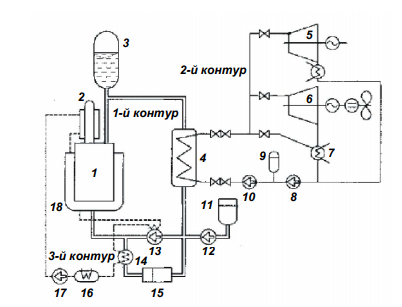
\includegraphics[width=4.56942in,height=3.48958in]{media/image1.png}
\caption{Принципиальная схема ледокольной ЯЭУ: 1-РУ; 2-приводы;
3-компенсатор давления; 4-парогенератор; 5-вспомогательный
турбогенератор; 6-главный турбогенератор; 7-главный конденсатор; 8-
конденсатный насос; 9-уравнительная цистерна; 10-питательный насос;
11-подпиточная система; 12-подпиточный насос; 13-центральный насос
первого контура; 14-холодильник фильтра; 15-ионнообменный фильтр;
16-холодильник 3\textsuperscript{го} контура; 17-циркуляционный насос
3\textsuperscript{го} контура; 18-бак металловодной защиты}
\end{figure}

\section{Выбор прототипа}

В развитии судовых РУ можно выделить 3 поколения судовых ядерных
энергетических установок (табл.1.1)

\begin{quote}
Таблица 1.1 -- Основные характеристики судовых РУ \cite{xlopkin}

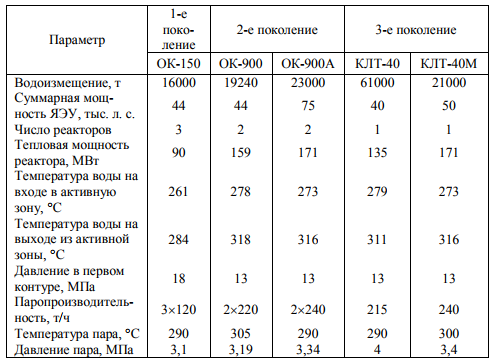
\includegraphics[width=5.59903in,height=4.08333in]{media/image2.png}
\end{quote}

В настоящее время последняя модификация РУ КЛТ-40 -- РУ КЛТ-40С
установлена на строящемся ПЭБ «Академик Ломоносов». Основное отличие РУ
КЛТ-40С от РУ КЛТ-40 -- переход от канальной активной зоны к кассетной.
КЛТ-40С отвечает последним требованиям по безопасности.

\begin{figure}[!h]
\center
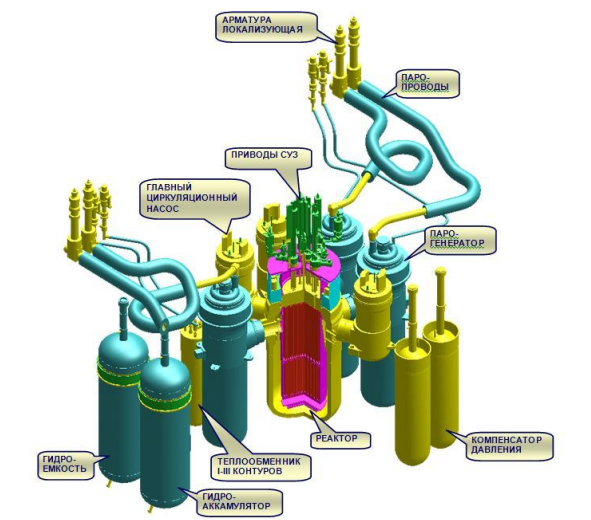
\includegraphics[width=4.56942in,height=3.48958in]{media/image3.png}
\caption{Общий вид РУ КЛТ-40С}
\end{figure}

\section{Анализ прототипа}

Реактор КЛТ-40С -- водо-водяной реактор с двухконтурной системой. Пар
второго контура, поступающий на турбину, изолирован от первого контура и
поэтому не является радиоактивным. Реакторная установка оснащена
надежными «пассивными» системами защиты, функциональность которой
базируется на законах природы - гравитации, конвекции, конденсации.
Благодаря этому, самосрабатывающие устройства системы безопасности не
зависят от электроснабжения.

Наука не стоит на месте, и благодаря этому разрабатываются современные
системы безопасности, внедряются новейшие достижения в области
металловедения, разрабатываются современные электротехнические,
автоматические и микроэлектронные устройства. Именно поэтому РУ КЛТ-40С
отвечает самым высоким требованиям безопасности. Технические
характеристики РУ КЛТ-40С приведены в таблице 1.2 \cite{deev}.

Таблица 1.2 -- Основные технические характеристик РУ КЛТ40-С

\begin{longtable}[]{@{}|l|l|@{}}
\toprule
Параметр, характеристики & Значение\tabularnewline
\midrule
\endhead
Количество РУ в составе энергоблока, шт. & 2\tabularnewline
Температура воды на выходе из реактора, \(\) & 317\tabularnewline
Давление 1-го контура при номинальной мощности, МПа &
12,7\tabularnewline
Температура воды на входе в реактор, \(\) & 294.7\tabularnewline
Энтальпия воды на входе в реактор, Дж/кг & 1439800\tabularnewline
Энтальпия воды на выходе из реактора, Дж/кг & 1311100\tabularnewline
Температура питательной воды, \(\) & 170\tabularnewline
Температура перегретого пара,\(\ \) & 285\tabularnewline
Давление пара за ПГ, МПа & 3.72\tabularnewline
Количество и мощность ЦНПК, кВт & 4х152\tabularnewline
Кампания активной зоны, лет & 2,5-3\tabularnewline
\bottomrule
\end{longtable}

На ПЭБ с РУ КЛТ40-С размещаются две паротурбинные установки
ТК-35/38-3,4. В состав ПТУ входят: паровая турбина, валоповоротное
устройство, система парораспределения, регулирования и защиты. Основные
технические характеристики данной ПТУ представлены в таблице 1.3
\cite{deev}

Таблица 1.3 -- Основные технические характеристик ПТУ ТК-35/38-3,4


\begin{longtable}[]{@{}|l|l|@{}}
\toprule
Наименование параметра & Значение\tabularnewline
\midrule
\endhead
Электрическая мощность, МВт & 35\tabularnewline
Параметры пара перед ПТУ,\(\ \) & 285\tabularnewline
Давление пара перед турбиной, МПа & 3.43\tabularnewline
Температура пара в регулируемом отборе, \(\) & 139.7\tabularnewline
Давление пара в регулируемом отборе, МПа & 0.357\tabularnewline
Давление в конденсаторе, МПа & 0.005\tabularnewline
Расход забортной воды на конденсатор, м\textsuperscript{3}/ч &
5000\tabularnewline
\bottomrule
\end{longtable}

Как уже отмечалось ранее, основное отличие модификации РУ КЛТ-40С от его
предшественника КЛТ-40 состоит в переходе от канальной активной зоны к
кассетной. В таблице 1.4 представлены основные параметры кассетной зоны
реактора КЛТ-40С
\clearpage
Таблица 1.4 -- Основные характеристики кассетной зоны реактора КЛТ-40С

\begin{longtable}[]{@{}|l|l|@{}}
	%\label{Основные характеристики кассетной зоны реактора КЛТ-40С}
\toprule
Параметр & Значение\tabularnewline
\midrule
\endhead
Количество ТВС, шт. & 121\tabularnewline
Диаметр АЗ, мм & 1219\tabularnewline
Высота АЗ H\textsubscript{аз}, мм & 1300\tabularnewline
Диаметр ТВЭЛа, мм & 6,8\tabularnewline
Шаг между ТВЭЛами, мм & 9.6\tabularnewline
Количество ТВЭЛов в АЗ, шт. & 12 342\tabularnewline
Продолжительность кампании, эффективных ч & 22 000\tabularnewline
\bottomrule
\end{longtable}

\chapter{Теплогидравлический расчет}
\section{Определение термического КПД паротурбинного цикла}

Расчет термического КПД реактора КЛТ-40С проводилось для паротурбинной
установки ТК-35/38-3,4. Основные параметра данной \nom{ПТУ}{паротурбинная установка} приведены в табл.1.3. Тепловая схема АППУ для данного реактора приведена на рис.2.1.

\begin{figure}[!h]
\center
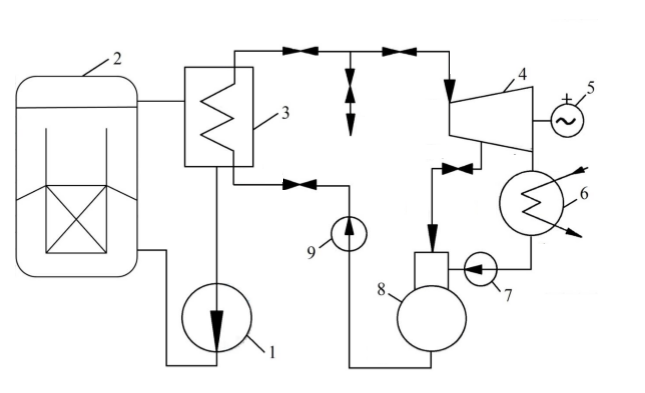
\includegraphics[width=6.49583in,height=3.95764in]{media/image4.png}
\caption{Расчетная тепловая схема \nom{АППУ}{атомная паропроизводящая установка} с реактором КЛТ-40С: 1 -
главный циркуляционный насос 1-го контура, 2 -- активная зона ядерного
реактора, 3 -- парогенератор, 4 - ЦВД турбины, 5 -- электрогенератор, 6
-- конденсатор, 7 -конденсатный насос, 8 - диаэратор, 9 -- питательный
насос}
\end{figure}

Данной тепловой схеме соответствует T-S диаграмма, приведенная на рис.
2.2.

\begin{figure}[!h]
\center
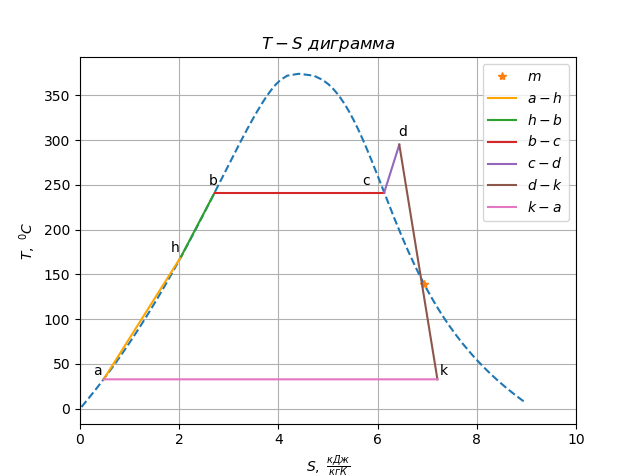
\includegraphics[width=0.9\textwidth]{media/image5.png}
\caption{T-S диаграмма : m -- точка регулируемого регенеративного отбора,
a-h -- участок регенеративного отбора, h-b -- экономайзерный участок,
b-c -- испарение, c-d -- пароперегрев, d-k -турбина, k-a - конденсация}
\end{figure}

Для построения данного графика использовались значения из таблицы 2.1,
полученные с помощью программы WaterSteamPro.

Таблица 2.1 - Значения теплофизических параметров на разных участках
тепловой схемы АППУ

Расчет КПД производился по формуле:

\[\eta_{3} = \eta_{0} + \left( \eta_{\infty} - \eta_{0} \right) \cdot \frac{n}{n + 1}\ ,\]

\flushleft где:
\begin{description}
	\item[${n}$] - число регенеративных отборов (в нашем случае \emph{n}=3),
	\item[$\eta_{0}$] - КПД, рассчитываемый без учета регенеративных отборов,
	\item[$\eta_\infty$] - КПД, рассчитываемый при идеальной
	регенерации (т.е. при бесконечном числе отборов).
\end{description}

\[\eta_{0} = 1 - T_{k} \cdot \frac{S_{d} - S_{a}}{i_{d} - i_{a}} = \ 0.3556\]

\[\eta_{\infty} = 1 - T_{k} \cdot \frac{S_{d} - S_{h}}{i_{d} - i_{h}} = 0.4011\]

Тогда получим:

\[\eta_{3} = 0,4149\]

КПД \nom{РУ}{реакторная установка} может быть рассчитан по формуле:

\[\eta_{Brutto} = \ \eta_{IT} \cdot \eta_{M} \cdot \eta_{EG} \cdot \eta_{oi} \cdot \eta_{3} = 0.2723\textrm{ ,} \]

где: 
\begin{description}
	\item[$\eta_{IT}$] = 0.98 -- коэффициент использования тепла,
	\item[$\eta_{M}$] = 0.97 -- механический КПД,
	\item[$\eta_{EG}$] = 0.98 -- КПД электрогенератора,
	\item[$\eta_{oi}$] = 0.7 -- внутренний относительный КПД турбины,
	\item[$\eta_{3}$] -- термический КПД, рассчитанный по формуле.
\end{description}

\section{Расчет тепловой мощности и построение T-Q диаграммы}

Зная электрическую мощность (таблица 1.3) и КПД РУ, вычислим тепловую
мощность установки:

\[\ Q =\frac{W}{\eta_{Brutto}} = 128.53\] МВт

Рассчитаем минимальный расход теплоносителя, необходимый для отвода
тепла Q в единицу времени:



\[G_1 = \frac{Q}{{i}_{1}} \cdot 3.6 = 998.7\]кг/с,

где \[{i}_{1}\] -- разность энтальпий 1-го контура (таблица 1.2)

Составим уравнение теплового баланса для 2-го контура:

\begin{equation}
Q = G_2\cdot(i_{ab} + i_{bc} + i_{cd})
\end{equation}

где ${i}_{ab}$ -- разность энтальпий на участке a-b (нагрев
воды 2-го контура до температуры насыщения), ${i}_{bc}$ --
разность энтальпий на участке испарения, ${i}_{cd}$ -- разность
энтальпий на участке пароперегрева (данные взяты из таблицы 2.1)

Тогда для расчета значения G­\textsubscript{2} получаем формулу:

\begin{equation}
G_2 =\frac{Q}{{i}_{ab} + {i}_{bc} + {i}_{cd}} = 57.92
\end{equation}


На основании полученных данных построим T-Q диаграмму (Рисунок 2.2) --
график, показывающий зависимости температур теплоносителя и рабочего
тела от переданного им тепла.

\begin{figure}[!h]
\center
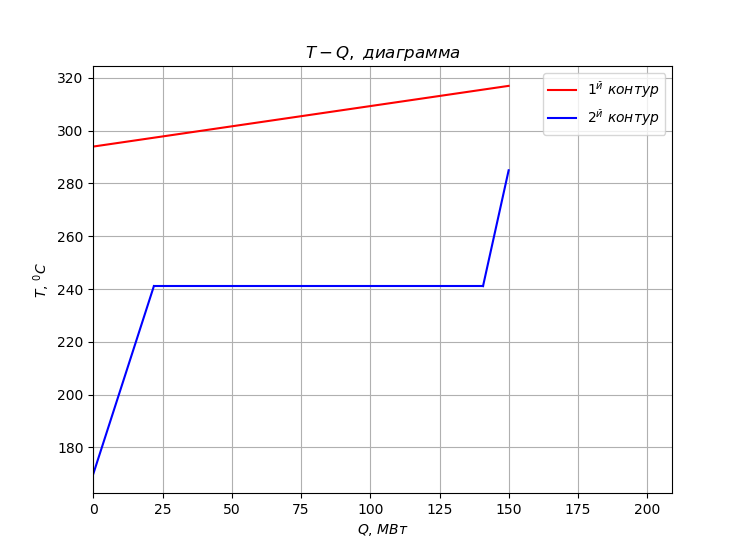
\includegraphics[width=16cm]{media/image7.png}
\caption{TQ-диаграмма}
\end{figure}

\section{Расчет дополнительных геометрических характеристик ТВС и
активной зоны}

\begin{figure}[!h]
\center
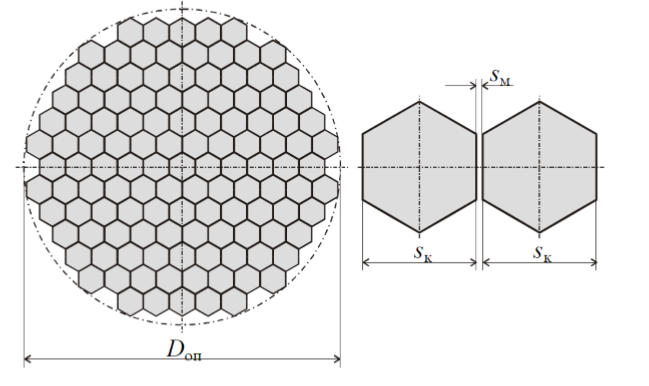
\includegraphics[width=14cm]{media/image8.png}
\caption{Компоновка ТВС в активной зоне \cite{deev}}
\end{figure}

В таблице 2.2 представлены основные технические характеристики ТВС и АЗ,
которые будут использоваться в дальнейшем.

Таблица 2.2 -- Основные характеристики АЗ

\begin{longtable}[]{@{}|p{10cm}|c|@{}} 
\toprule
Наименование параметра & Значение\tabularnewline
\midrule
\endhead
Тип и форма ТВС & Чехловая с вытеснителем \tabularnewline
Форма вытеснителя & Шестигранная\tabularnewline
Диаметр твэла d\textsubscript{\nom{твэл}{тепловыделяющий элемент}}, мм & 6.8\tabularnewline
Эквивалентный диаметр компенсатора распухания d\textsubscript{комп}, мм
& 2.52\tabularnewline
Шаг решетки твэлов s,мм & 9.6\tabularnewline
Длина активной части твэла H\textsubscript{АЗ}, мм & \centering 1300\tabularnewline
Размер чехла ТВС под ключ s\textsubscript{k}, мм & 96\tabularnewline
Расстояние между ТВС s\textsubscript{м}, мм & 2\tabularnewline
Толщина чехла ТВС $\delta_{tvs},\ mm$ & 1.65\tabularnewline
Количество ТВС, шт & 121\tabularnewline
Количество твэлов N\textsubscript{твэл}, шт & 69\tabularnewline
Количество СВП $\O$ 6.8 мм N\textsubscript{СВП1,} шт & 9\tabularnewline
Количество СВП $\O$ 4.5 мм N\textsubscript{СВП2,} шт & 6\tabularnewline
Толщина оболочки СВП1 $\delta$\textsubscript{СВП1,} мм & 0.5\tabularnewline
Толщина оболочки СВП2 $\delta$\textsubscript{СВП2,} мм & 0.45\tabularnewline
Количество пэлов в кластере вытеснителя, мм & 7\tabularnewline
Толщина оболочки пэла $\delta$\textsubscript{пэл}, мм & 0.5\tabularnewline
Площадь поперечного сечения вытеснителя S\textsubscript{в},
мм\textsuperscript{2} & 689\tabularnewline
Эквивалентный диаметр компенсатора распухания d\textsubscript{комп,} мм
& 2.52\tabularnewline
\bottomrule
\end{longtable}

По данным таблицы 2.2 найдем геометрические параметры АЗ:

описанный диаметр АЗ:

\[D_{op} = \sqrt{\frac{2 \cdot \sqrt{3}}{\pi}N_{TVS}}(S_{k} + S_{m}) = 1132\textrm{ мм}\]

относительный шаг решетки:

\[x = \ \frac{s}{d_{tvel}} = 1.41\]
\begin{center}
эквивалентный диаметр треугольной решетки:

\[d_{ekv} = \ d_{tvel}\left( \frac{2\sqrt{3}}{\pi} \cdot x^{2} - 1 \right)= 8.14 \textrm{ мм}\]


площадь поперечного сечения кассеты:

\[\emph{S­\textsubscript{tvs}} =S­\textsubscript{tvs}\frac{\sqrt{3}}{2} \cdot (s_{k} - 2 \cdot \delta_{tvs}) ^2= 7750.2 \textrm{ мм}^2\]

площадь проходного сечения:


\[\emph{S­\textsubscript{tn }}=S_{tvs} - \ \pi \cdot \left( N_{tvel}\frac{{d_{tvel}}^{2}}{4} + \ N_{svp1}\frac{{d_{svp1}}^{2}}{4} + \ N_{svp2}\frac{{d_{svp2}}^{2}}{4} \right) - S_{v}\]

\[\emph{S­\textsubscript{тн }}= 4133.06 \textrm{мм}\textsuperscript{2}\]

обогреваемый периметр:

\[d_t = N_{tvel} \ \pi \ d_{tvel}=1.474 \textrm{ м}\]
эквивалентный диаметр АЗ:

\[D_{ekv} = \ \sqrt{\frac{2\sqrt{3}}{\pi}\ N_{tvs}}\ \left( s_{k} + s_{m} \right) = 1131.98\ \textrm{мм}\]

объем АЗ:


\[V_{az} = \ \frac{\pi\ H_{az}{D_{ekv}}^{2}}{4} = 1.308\ \textrm{м}\textsuperscript{3}\]
\end{center}

\section{Расчет средних тепловых характеристик активной зоны}

Удельная энергонапряженность АЗ:

\[q_{v} = \ \frac{Q_{t}}{V_{az}} = 98.243\ \frac{MVt}{m^{3}}\]

Средняя тепловая мощность ТВС:

\[Q_{tvs} = \ \frac{K_{Q}Q_{t}}{N_{tvs}} = 1.04 \textrm{ МВт,} \] 
где \emph{K\textsubscript{Q }}= 0.98 -- коэффициент, учитывающий долю тепла,
выделяющегося в твэлах.

Средний линейный тепловой поток от твэлов:

\[q_{lsr} = \frac{Q_{TVS}}{n_{tvel}H_{az}} = 11.6 \frac{\textrm{ кВт}}{\textrm{м}}\]

Средняя плотность теплового потока на поверхности твэлов:

\[q_{sr} = \frac{Q_{TVS}}{F_{to}} = \frac{q_{lsr}}{\pi d_{tvel}} = 543.25 \frac{\textrm{ кВт}}{\textrm{м}^2}\]

\section{Расчет распределения температур по высоте для ТВС с
максимальным энерговыделением}

\subsection{Распределение плотности теплового потока по высоте твэла
для ТВСМ}

В первом приближении коэффициенты неравномерности возьмем следующие:

\[k_{r} = 1.42\] \[k_{z} = 1.36\]

Соответственно \[\emph{k\textsubscript{v}} =k_{r} \cdot k_{z} = 1.9312\]

Исходя из данных коэффициентов неравномерности найдем высоту и радиус
активной зоны с учетом отражателя:

\[k_{z} = \frac{q_{0,z}}{\frac{1}{H}\int_{-H/2}^{H/2}{q_{0,z}\cos{( \frac{\pi z}{H_{ef}} )dz}}} =\frac{H}{H_{ef}}\frac{\pi}{2}\frac{1}{\sin( \frac{\pi H}{2H_{ef}})} = k_{z}\sin( \frac{\pi H}{2H_{ef}}) = \frac{\pi H}{2H_{ef}}\]


\[H_{ef} = 1.55\ \textrm{м}\]

\[k_{r} = \frac{q_{0,z}}{\frac{1}{\pi R^{2}}\int_{0}^{R}{q_{0,r}{\left( \xi_{0}\frac{r}{R_{ef}} \right)dr}}} = \frac{R}{R_{ef}}\frac{\xi_{0}}{2\left( \xi_{0}\frac{R}{R_{ef}} \right)} = > 2k_{r}\left( \xi_{0}\frac{R}{R_{ef}} \right) = \xi_{0}\frac{R}{R_{ef}}\]

\[R_{ef} = 0.9\ \textrm{м}\]

Распределения плотности теплового потока выглядит следующим образом:

\[q\left( z \right) = q_{\max}\cos \pi\frac{z}{H_{eff}} \]

\[q_{l}\left( z \right) = q_{lmax}\cos \pi\frac{z}{H_{eff}} \ ,\]

где \[q_{\max} = \ \emph{k\textsubscript{v} q\textsubscript{ср} = }1.049 \frac{\textrm{ МВт}}{\textrm{м}^{2}}\],
\[q_{lmax} = k_{v}q_{lsr} = 11.61\ \frac{\textrm{КВт}}{\textrm{м}} , \emph{z} \in-\textrm{[}\frac{H_{az}}{2};\ \frac{{\ H}_{az}}{2}\textrm{]} \]

\begin{figure}[!h]
\center
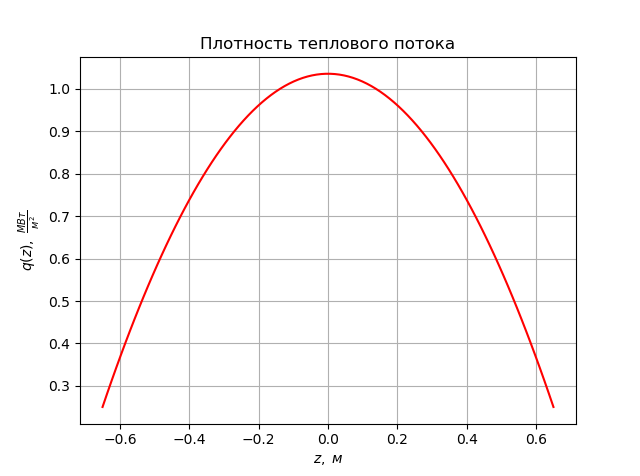
\includegraphics[height=10cm]{media/image9.png}
\caption{График распределения плотности теплового потока по высоте
твэла для ТВСМ}
\end{figure}

\subsection{Распределение температур во высоте ТВСМ}

Распределение температур теплоносителя по высоте описывается формулой
(2.20):

\[t_{v} = t_{v} + \frac{k_{G}P_{t}q_{\max}}{k_{Q}G_{tn}S_{p}}\int_{-_{\frac{H_{az}}{2}}}^{z}{cos\left( \pi\frac{z}{H_{eff}} \right)dz}\]

Распределение температуры внешней оболочки твэла:

\[t_{ob.n}\left( z \right) = t_{zh}\left( z \right) + q\left( z \right)R_{\alpha},\]

где \[R_{\alpha} = \ \frac{1}{\alpha}\] .

Для расчета коэффициента теплоотдачи будем использовать следующие
формулы:

\[Nu =  0,0165 + 0,02\left( 1 - \frac{0,91}{x^{2}} \right)x^{0,15} Re^{0,8}\Pr^{0,4}\]

\[w = \ \frac{k_{G}G_{1}k_{r}}{\rho S_{tn}N_{tvs}} = 3.73\ \frac{\textrm{м}}{\textrm{с}}\ ,\]

\flushleft $k_{G}$ = 0,93 \textrm{ -- коэффициент протечек.}
\[Re = \frac{wd}{\nu} = 2.52 \cdot 10^{5}\]

Тогда получим коэффициент теплоотдачи:

\[\alpha\  = \frac{Nu\lambda}{d_{ekv}} = 3.74 \cdot 10^{4}\ \frac{Vt}{m^{2}K}\]

Распределение температуры внутренней оболочки твэла:

\[R_{ob} = \frac{\ln\left( \frac{d_{tvel}}{d_{tvel} - 2\delta_{ob}} \right)}{2\pi\lambda_{ob}},\]

где $\lambda_{ob}$ = 18$\frac{\textrm{Вт}}{\textrm{м} \cdot K}$ -- теплопроводность
оболочки твэла

\[t_{ob.vn}\left( z \right) = t_{ob.n}\left( z \right) + q_{l}\left( z \right)R_{ob}\]


Распределение температуры топливного сердечника с компенсатором
распухания:

\[t_{ts.t}\left( z \right) = t_{ob.vn}\left( z \right) + q\left( z \right)R_{t.s}\ ,\]

где $\lambda_{t}$ = 35$\frac{\textrm{ Вт}}{\textrm{м} \cdot K}$ -- теплопроводность
ThO\textsubscript{2} в силуминовой матрице в начале кампании

\[R_{t.s} = \frac{d_{tvel}}{4\lambda_{t} 1 - \left( \frac{d_{komp}}{d_{t.s}} \right)^{2} }\left\{ 1 - \left( \frac{d_{komp}}{d_{t.s}} \right)^{2} 1 - 2\ln\left( \frac{d_{t.s}}{d_{komp}} \right)  \right\}.\]

Все вышеперечисленные зависимости температур представлены на рисунке 2.6

\begin{figure}[!h]
\center
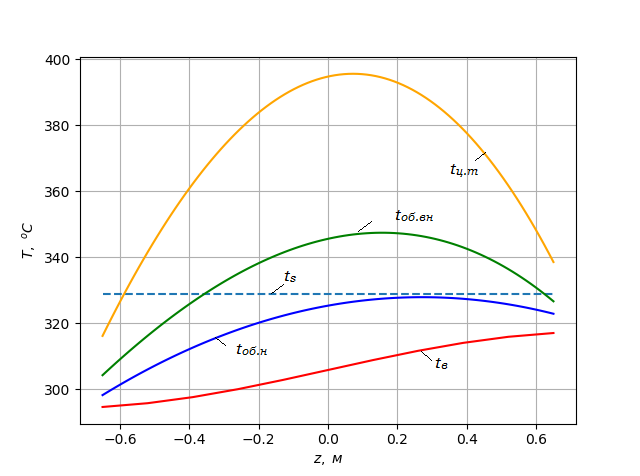
\includegraphics[width=6in]{media/image10.png}
\caption{График распределения температур по высоте ТВСМ:
t­\textsubscript{в} - температура теплоносителя, t­\textsubscript{об.н}
-- температура наружной оболочки, t­\textsubscript{об.н} -- температура
внутренней оболочки, t­\textsubscript{т.ц} -- температура топливной в
центре сердечника, t­\textsubscript{s} -- температура насыщения 329.04
$^\circ C$.}
\end{figure}

Таблица 2.3 -- Максимальные температуры в \nom{ТВСМ}{сборка твэлов с максимальным энерговыделением}

\begin{longtable}[]{@{}|C{4cm}|C{4cm}|@{}} 
\toprule
& t\textsubscript{max,} $^\circ C$.\tabularnewline
\midrule
\endhead
t\textsubscript{об.н} & 328.79\\ \hline
t\textsubscript{об.вн} & 347.80\\ \hline
t\textsubscript{ц.т} & 395.98\\ 
\bottomrule
\end{longtable}

\clearpage

\section{Оценка коэффициента запаса до кризиса теплообмена}

Учет отличия теплового диаметра $d_{t}$ стандартной ячейки от базового
значения:

\begin{equation}
K_{1} = \left( \frac{d_{t}}{9,36} \right)^{- \frac{1}{3}} = 1,112
\end{equation}


Учет относительного шага расположения стержней:

\begin{equation}
K_{2} = 0,2 + 0,57\left( \frac{s}{d} \right) = 1.0037
\end{equation}


Учет влияния на критический тепловой поток входных условий сборки:

\begin{equation}
K_{3} = 1 + 0,6\exp{\left( - \frac{0,01L}{d_{t}} \right) = 1.089}
\end{equation}


Учет турбулизирующего воздействия на кризис кипения дистанционирующих
решеток:

\begin{equation}
K_{4} = 1 + Aexp\left( - \frac{0.01Z}{d_{t}} \right) = 1.2
\end{equation}

\begin{equation}
K = K_{1}K_{2}K_{3}K_{4}K_{5} = 1,136
\end{equation}

\begin{quote}
\[q_{kr} = q_{kr.tab}K\]
\end{quote}


Табличные значения КТП для
\[P = 12,7\ \textrm{МПа}\ \textrm{и}\ \rho w = 2367\frac{\textrm{кг}}{\textrm{м} \cdot \textrm{с}}\]


Таблица 2.4 -- значения КТП

\begin{longtable}[]{@{}|c|c|c|c|c|c|c|c|c|c|@{}}
\toprule
x & -0,4 & -0,3 & -0,2 & -0,1 & 0 & 0,1 & 0,2 & 0,3 & 0,4\tabularnewline
\midrule
\endhead
q\textsubscript{кр.таб}, МВт & 6.48 & 5.60 & 4.46 & 3.29 & 2.47 & 1.85 &
1.29 & 0.81 & 0.47\tabularnewline
q\textsubscript{кр}, МВт & 10.01 & 8.64 & 6.88 & 5.08 & 3.81 & 2.85 &
1.99 & 1.25 & 0.72\tabularnewline
\bottomrule
\end{longtable}

На график (Рисунок 2.7) нанесены значения КТП с учетом поправок, взятые
из таблицы 2.4, а также кривые
\[q_{kr}\left( 1 \pm \sigma_{kv} \right)\], которые характеризуют
возможное расхождение между расчетными значениями и экспериментальными
данными.

\[\sigma_{kv} = 0,15\] -- среднеквадратичное отклонение данных
экспериментов от расчетной формулы или данных таблицы.

\begin{figure}[!h]
\center
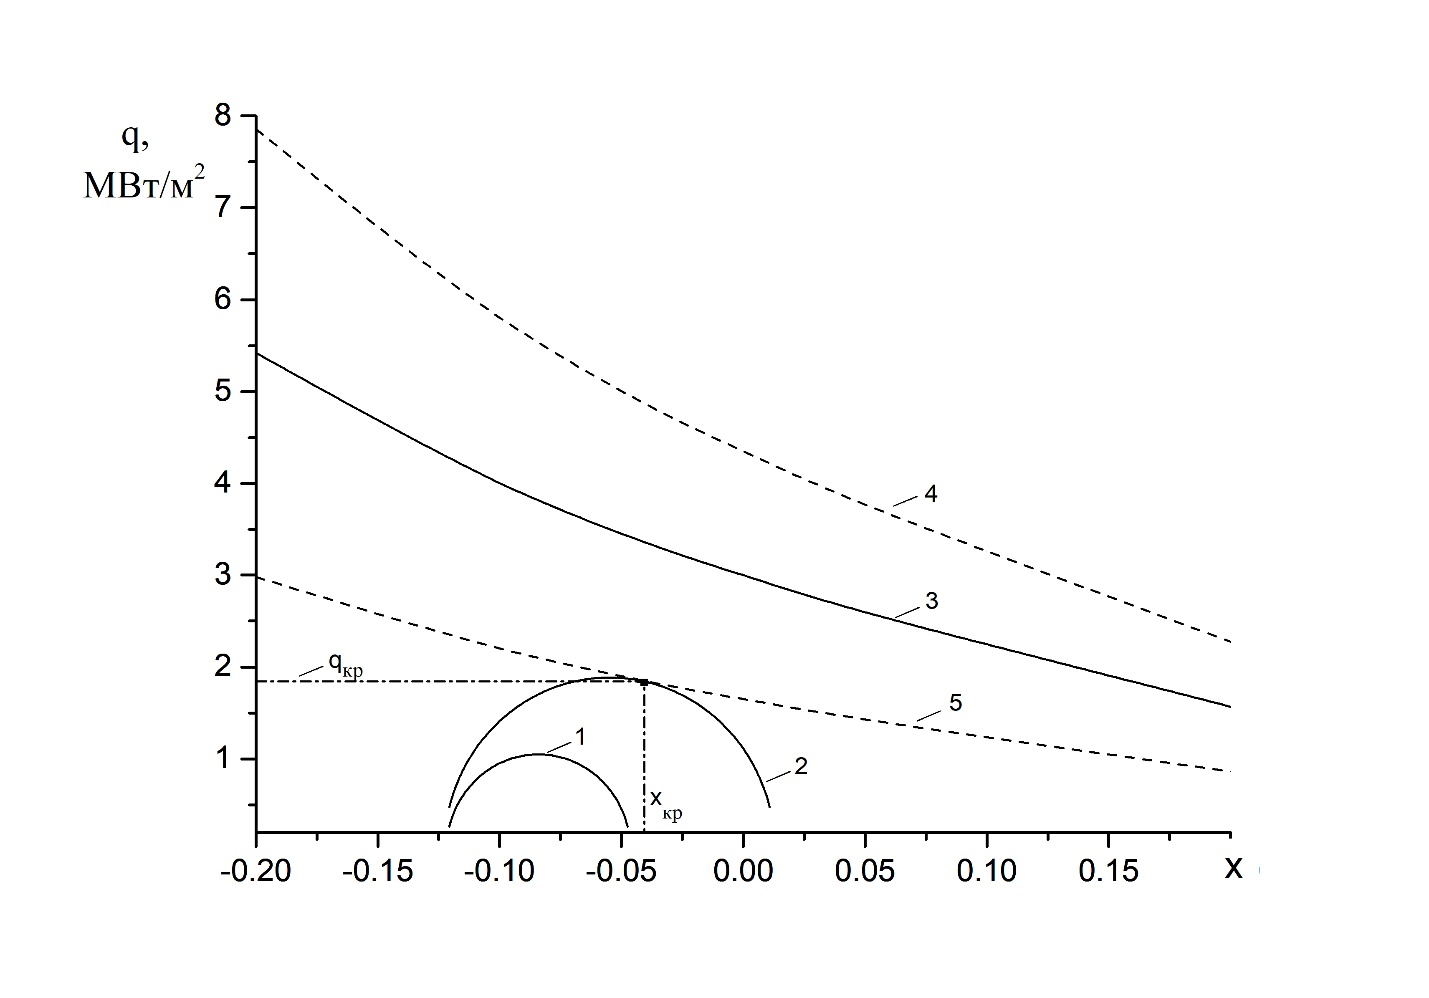
\includegraphics[width=6.49583in,height=4.53750in]{media/image11.png}
\caption{График определения запаса до кризиса теплообмена: 1 --
распределение плотности теплового потока в ТВСМ в номинальном режиме
работы реактора; 2 -- то же, но при увеличении q в 1.8 раза; 3 --
расчетные значения КТП согласно табличному методу; 4,5 -- то же с учетом
возможных отклонений расчетных значений от экспериментальных данных.}
\end{figure}

Из данного рисунка видно, что в точке (\emph{x\textsubscript{кр,}
q\textsubscript{кр}}) кривые 2 и 5 касаются друг друга.

Это означает, что при следующих параметрах \emph{x\textsubscript{кр}} =
-0.04, \emph{q\textsubscript{кр}} = 1.844 существует вероятность
возникновения кризиса теплообмена который может произойти в сечении
ТВСМ, находящемся на расстоянии около 0.8 м от входа в сборку
(\[z_{kr} \approx 1.1\ m\]).

\[K_{zap} = 1.8\]

\section{Расчет гидравлических сопротивлений ТВС}

Полные потери давления при движении теплоносителя в каналах АЗ реактора
вычисляются по следующей формуле:

\[p = p_{tr} + \sum_{}^{}{p_{m} \pm p_{usk} \pm p_{niv}}\]

Коэффициент сопротивления трения:

\[\xi_{0} = {(1,82lgRe - 1,64)}^{- 2} = 0.016\]

\[\frac{\xi}{\xi_{0}} = 1,10 + 0,18\left( x - 1 \right) = 1.17\]

\[\xi = 0.019\]

Перепад давления из-за трения:

\[p_{tr} = \xi\frac{L}{d_{g}}\frac{\rho w^{2}}{2} = 7287\ Pa\]

Таблица 2.5- Коэффициенты местных сопротивлений:

\begin{longtable}[]{@{}llllll@{}}
\toprule
$\zeta$\textsubscript{вх} & $\zeta$\textsubscript{вых} & $\zeta$\textsubscript{н.р} &
$\zeta$\textsubscript{в.р} & 5$\zeta$\textsubscript{др} &
$\Sigma$$\zeta$\textsubscript{м}\tabularnewline
\midrule
\endhead
6 & 4 & 2 & 3 & 0.83 & 15.83\tabularnewline
\bottomrule
\end{longtable}

Падение давления на местных сопротивлениях:

\[p_{m} = \frac{\rho w^{2}}{2}\sum_{}^{}{\xi_{m} = 38.574\ kPa}\]

Потери напора на ускорение:

\[p_{usk} = \left( \rho w \right)^{2}\left( \frac{1}{\rho_{k}} - \frac{1}{\rho_{n}} \right) = 369\ Pa\]

Нивелирный напор:

\[p_{niv} = \left( \rho_{n} - \rho_{k} \right)gH = 339\ Pa\]

Полная потеря давления:

\[p = p_{tr} + p_{m} + p_{usk} - p_{niv} = 54.69\ kPa\]

Затраты мощности на прокачку теплоносителя через активную зону:

\[N = \frac{Vp}{\eta_{n}} = 291.44\ kVt\]

Где V -- объемный расход теплоносителя, \[\eta_{n}\] -- \nom{КПД}{коэффициент полезного действия}
циркуляционного насоса.

Затраты мощности на прокачку теплоносителя составляет менее 0.83\% от
электрической мощности реактора.

\chapter{Нейтронно-физический расчет ядерного реактора}

\section{Формирование активной зоны реактора}

Активная зона проектируемого реактора имеет кассетную структуру. Кассеты
имеют форму шестигранников, внутри которых находятся тепловыделяющие
элементы. Активная зона реактора тепловой мощностью 128.53 МВт (глава 2)
состоит из 121 ТВС, описанный диаметр -- 1200 мм, высота -- 1300 мм.

\begin{figure}[!h]
\center
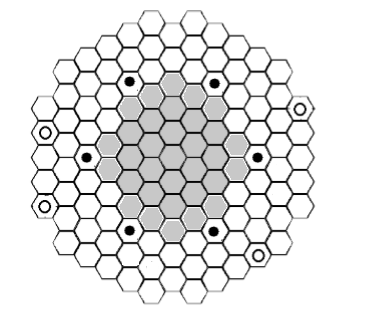
\includegraphics[width=4.43750in,height=3.83293in]{media/image12.png}
\caption{Компоновка активной зоны : - ТВС центральной зоны; - ТВС
периферийной зоны; - ТВС со стержнем АЗ; - ТВС с пустым каналом}
\end{figure}

Таблица 3.1 - Типы и состав ТВС активной зоны


\begin{longtable}[]{@{}lllll@{}}
\toprule
Тип ТВС & Число ТВС & Число "тяжелых" / "легких" твэлов & Число СВП-1 &
Число СВП-2\tabularnewline
\midrule
\endhead
ТВС центральной зоны & 33 & 69 / - & 9 & 6\tabularnewline
ТВС периферийной зоны & 78 & 18 / 51 & 9 & 6\tabularnewline
ТВС со стержнем АЗ & 6 & 18 / 51 & 9 & 6\tabularnewline
ТВС с пустым каналом & 4 & 18 / 51 & 9 & 6\tabularnewline
\bottomrule
\end{longtable}

\begin{figure}[!h]
\center
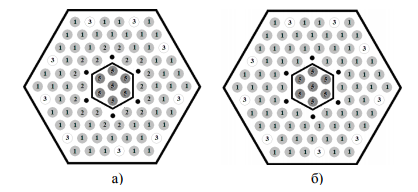
\includegraphics[width=4.59375in,height=2.10972in]{media/image13.png}
\caption{Схема размещения элементов в ТВС периферийной (а) и
центральной (б) зоны: 1 -- «тяжелые» твэлы; 2 -- «легкие» твэлы; 3 --
СВП-1; 4 -- СВП-2; 5 -- пэлы}
\end{figure}

\begin{figure}[!h]
\center
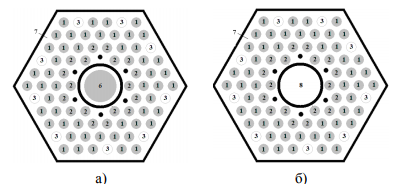
\includegraphics[width=4.15625in,height=2.00000in]{media/image14.png}
\caption{Схема размещения элементов в ТВС со стержнем АЗ (а) и
пустым каналом (б): 1 -- «тяжелые» твэлы; 2 -- «легкие» твэлы; 3 --
СВП-1; 4 -- СВП-2; 6 -- стержень АЗ; 7 -- теплоноситель; 8 -- пустой
канал}
\end{figure}

\section{Подготовка макроскопических параметров для стационарного и
динамических расчетов}


Для последующих \nom{НФР}{нейтронно-физический отсчет} расчетов необходимо знать двухгрупповые
макроскопические параметры для каждого типа ТВС. Для твэлов с подвижными
элементами (пэлы, стержни АЗ) необходимо знать два набора
макроскопических параметров -- с поднятыми и опущенными стержнями.

Расчет данных параметров производится по спектральной программе GETERA с
использованием полиячейки (ТВС), каждый отдельный элемент (моноячейка)
-- многозонная ячейка. Для описания полиячейки необходимо знать позонную
концентрацию нуклидов, число ячеек и матрицу вероятнойстей перехода
нейтронов между отдельными моноячейками, а также температуры зон ячеек.

Для расчета концентрации нуклидов применим следующую формулу:

\(\rho_{i} = \varepsilon_{i}N_{A}\frac{\gamma_{i}}{M_{r}^{i}}\) ,

где \(N_{A}\) -- число Авогадро, \(M_{r}^{i}\) -- молярная масса,
\(\varepsilon_{i}\) -- объемная доля, \(\gamma_{i}\) -- плотность
вещества.

Применим следующие допущения:

\begin{enumerate}
\item
  Не будем учитывать наличие в материалах элементов с малой
  концентрацией или изотопов, обладающих малым макроскопическим сечением
  взаимодействия с нейтронами.
\item
  Будем считать, что температура одинакова в пределах одной зоны.
\item
  Не будем учитывать влияние компенсатора распухания и материал чехла
  ТВС на расчеты.
\end{enumerate}

\begin{quote}
Исходя из вышеперечисленных предположений, получим ядерные концентрации,
представленные в таблице 3.2

Таблица 3.2 -- Концентрация веществ, содержащихся в АЗ
\end{quote}

\begin{longtable}[]{@{}l@{}}
\toprule
ТВЭЛ-Т\tabularnewline
\midrule
\endhead
Нуклид\tabularnewline
Th\textsuperscript{232}\tabularnewline
U\textsuperscript{233}\tabularnewline
O\tabularnewline
ТВЭЛ-Л\tabularnewline
Нуклид\tabularnewline
Th\textsuperscript{232}\tabularnewline
U\textsuperscript{233}\tabularnewline
O\tabularnewline
Оболочка ТВЭЛа, СВП, ПЭЛа (сплав Э-110)\tabularnewline
Нуклид\tabularnewline
Zr\tabularnewline
Силуминовая матрица\tabularnewline
Нуклид\tabularnewline
Al\tabularnewline
Si\tabularnewline
\bottomrule
\end{longtable}

\begin{longtable}[]{@{}l@{}}
\toprule
СВП\tabularnewline
\midrule
\endhead
Нуклид\tabularnewline
Gd\textsuperscript{155}\tabularnewline
Gd\textsuperscript{157}\tabularnewline
O\tabularnewline
Al\tabularnewline
Сердечник АЗ\tabularnewline
Поглотитель\tabularnewline
Нуклид\tabularnewline
B\textsuperscript{10}\tabularnewline
B\textsuperscript{11}\tabularnewline
C\tabularnewline
Оболочка\tabularnewline
Нуклид\tabularnewline
Ni\tabularnewline
Cr\tabularnewline
Воздух\tabularnewline
Нуклид\tabularnewline
N\tabularnewline
O\tabularnewline
Сердечник ПЭЛа\tabularnewline
Нуклид\tabularnewline
B\textsuperscript{10}\tabularnewline
B\textsuperscript{11}\tabularnewline
C\tabularnewline
\bottomrule
\end{longtable}

Далее для программы GETERA необходимо рассчитать матрицу перетечки между
моноячейками :

\(P_{ij} = \frac{S_{ij}}{S_{i}}\),

где \(P_{ij}\) -- вероятность перехода нейтрона из ячейки
\emph{i} в ячейку \emph{j}, \(S_{ij}\) -- площадь поверхности,
смежной между обоими типами поверхности, \(S_{i}\) -- площадь
поверхности ячеек типа \emph{i}. Была рассчитана матрица вероятностей
(таблица 3.3).

Таблица 3.3 -- матрица вероятностей для P\emph{\textsubscript{ij}} ТВС

\begin{longtable}[]{@{}ll@{}}
\toprule
Тип ячейки & P\emph{\textsubscript{ij}}\tabularnewline
\midrule
\endhead
& ТВЭЛ-1\tabularnewline
ТВЭЛ-1 & 0.5359\tabularnewline
ТВЭЛ-2 & 0.2963\tabularnewline
СВП-1 & 0.8148\tabularnewline
СВП-2 & 0.0000\tabularnewline
ПЭЛ/АЗ & 0.0000\tabularnewline
КМ & 0.4783\tabularnewline
\bottomrule
\end{longtable}

\section{Уточнение теплофизического расчета}

После получения в программе GETERA всех необходимых макропараметров
подставим их в программу SKETCH. Она позволяет получить данные о
распределении нейтронного поля и энерговыделения в активной зоне на
начало кампании реактора. Так же из данной программы находим новое
распределение коэффициентов неравномерности по высоте
(\emph{k\textsubscript{z}}) и по радиусу (\emph{k\textsubscript{r­}}). С
данными коэффициентами пересчитываем теплофизический расчет и получаем
новое распределение теплового потока и температур по высоте. Далее
заново делаем расчет по программе GETERA c новыми полученными
температурами. Данную процедуру делаем до тех пор, пока коэффициенты
неравномерности не перестанут меняться. В данном случае количество
итераций получилось равное двум.

На графиках 3.3 и 3.4 показано окончательное распределение плотности
теплового потока и температур в ТВСМ по высоте соответственно.

\begin{figure}[!h]
\center
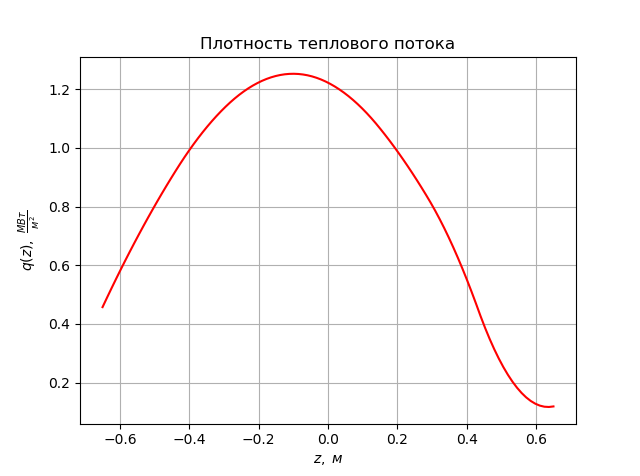
\includegraphics[width=5.11811in,height=3.80659in]{media/image15.png}
\caption{График распределения плотности теплового потока по высоте
для ТВСМ}
\end{figure}

\begin{figure}[!h]
\center
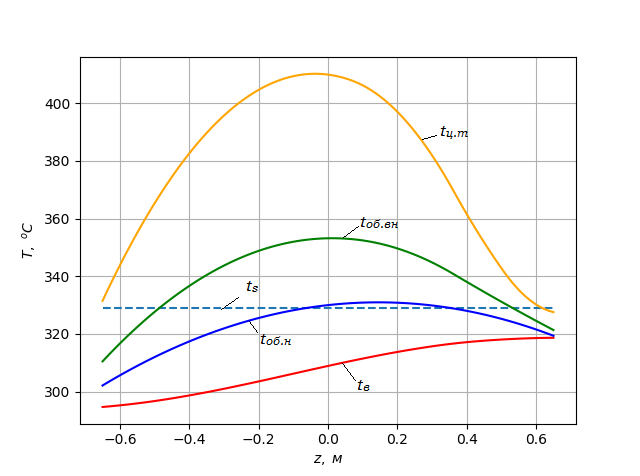
\includegraphics[width=5.11811in,height=3.80712in]{media/image16.png}
\caption{График распределения температур по высоте для ТВСМ}
\end{figure}

Таблица 3.4 -- Максимальные температуры В ТВСМ

\begin{longtable}[]{@{}ll@{}}
\toprule
& t\textsubscript{max,} $^\circ C$.\tabularnewline
\midrule
\endhead
t\textsubscript{об.н} & 331.66\tabularnewline
t\textsubscript{об.вн} & 353.83\tabularnewline
t\textsubscript{ц.т} & 420.05\tabularnewline
\bottomrule
\end{longtable}

\section{Расчет длительности кампании и выгорания топлива}

Для расчета длительности кампании была сформирована полиячейка,
состоящая из ТВС центральной и периферийной сборок. С помощью программы
GETERA было рассчитано максимальное выгорание топлива и длительность
кампании реактора (рисунок 3.5 и рисунок 3.6 соответственно).

\begin{figure}[!h]
\center
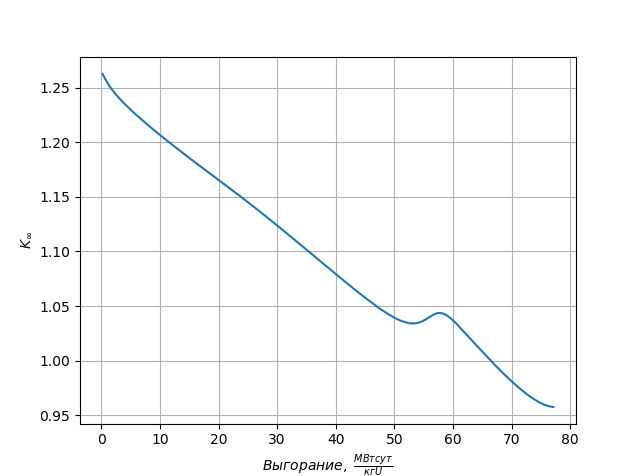
\includegraphics[width=5.11811in,height=3.80659in]{media/image17.png}
\caption{График зависимость \emph{$k_\infty$} от выгорания}
\end{figure}

\begin{figure}[!h]
\center
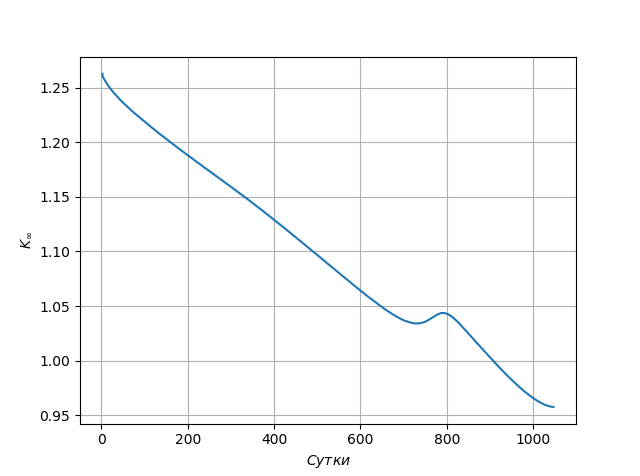
\includegraphics[width=5.11811in,height=3.80659in]{media/image18.png}
\caption{График зависимость \emph{$k_\infty$} от
количества суток}
\end{figure}

Как видно из данных графиков длительность кампании реактора $\approx$ 900 суток,
а максимальное выгорание топлива составляет
66.3\(\ \frac{MVt \cdot sut}{kg\ U}\).

\chapter{Расчет биологической защиты}
\section{Постановка задачи}

\section{Постановка задачи}

\begin{figure}[!h]
	\center
	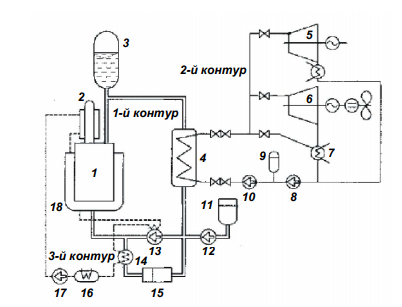
\includegraphics{media/image1.png}
	\caption{Принципиальная схема ледокольной ЯЭУ: 1-РУ; 2-приводы;
		3-компенсатор давления; 4-парогенератор; 5-вспомогательный
		турбогенератор; 6-главный турбогенератор; 7-главный конденсатор; 8-
		конденсатный насос; 9-уравнительная цистерна; 10-питательный насос;
		11-подпиточная система; 12-подпиточный насос; 13-центральный насос
		первого контура; 14-холодильник фильтра; 15-ионнообменный фильтр;
		16-холодильник 3\textsuperscript{го} контура; 17-циркуляционный насос
		3\textsuperscript{го} контура; 18-бак металловодной защиты}
\end{figure}




\bibliographystyle{plain}
\bibliography{tolik}
\end{document}
